\label{sec:vor}Für das Vorgehen zur Lösung der in Abschnitt \ref{sec:aufg} genannten Aufgaben zentral sind die folgenden Bereiche:
\begin{enumerate}[label=(\roman*)]
	\item Die Interaktion mit dem Benutzer, der das Programm steuert, d.\,h.
	\begin{itemize}
	\item das Entwerfen von Gesten für die verschiedenen Zwecke, die intuitiv und eingängig, leicht ausführbar und gut voneinander unterscheidbar sind sowie 
	\item das Auszeichnen einer getrackten Person als \glqq{}Master\grqq{} (i.\,F. zum Teil auch so bezechnet), der als einziger das Programm steuert.
	\end{itemize}
	\item Die technische Umsetzung, d.\,h.
	\begin{itemize}
	\item das konkrete Verfahren zur Auszeichnung einer Person als Master,
	\item damit verbunden das korrekte Wiedererkennen der ausgezeichneten Person und die Verhinderung der Programmsteuerung durch andere,
	\item das korrekte Erkennen und Werten von Gesten der ausgezeichneten Person und
	\item die Einbindung der Software, die all dies leistet, in die bereits bestehende Applikation.
	\end{itemize}
	\end{enumerate}
In diesem Abschnitt werden die unmittelbaren wichtigen Beobachtungen und Überlegungen vorgestellt, die sich aus der Aufgabenstellung und dem Versuchsaufbau ableiten lassen.\par 
Von der formulierten Aufgabe ausgehend kann abstrahierend zwischen zwei primitiven Steuerungsmodi unterschieden werden:
\begin{itemize}
	\item Einem Modus, in dem die Kamera verschoben und rotiert werden kann und 
	\item einem Modus, in dem Objektmanipulationen möglich sind.
\end{itemize} 
Der Benutzer sollte sich zu jedem Zeitpunkt der Programmausführung nur in maximal einem dieser Modi aufhalten, d.\,h. gleichzeitige Kamera- und Objektmanipulationen sind ausgeschlossen. Diese Vereinfachung gestattet einerseits die Verwendung von weniger komplexen Gesten, andererseits besitzt eine solche simultane Manipulation keine vordergründige praktische Relevanz und kann auch als mit dem Prinzip der Einfachheit in Konflikt stehend angesehen werden. Zusätzlich bietet sie als Ansatz bereits eine geeignete Kapselung, da zum Beispiel Rotationsparameter berechnet werden können und dann nur noch entschieden werden muss, ob sie auch die Kamera oder ein Objekt anzuwenden sind, je nach Modus. Dies erlaubt es gegebenenfalls die Anzahl der verwendeten Gesten weiter zu reduzieren, wenn für die verschiedenen Modi Gesten wiederverwendet werden.\par
Die Kinect ermöglicht ein Tracking des gesamten Körpers für mehrere Personen (vgl. Abschnitt \ref{sec:kinect}). Für die vorgesehene Anwendung ist jedoch nur ein Teil dieses Datenspektrums relevant:
\begin{itemize}
\item Der Hauptteil der Funktionalität \glqq{}Steuerung durch eine bestimmte Person\grqq{} betrifft nur die Tracking-Daten eines Benutzres. Eine genaue Auswertung weiterer sich im Raum befindlicher Personen und ihrer Skelette ist zumeist unnötig.
\item Die Gesten, die für den gegebenen Anwendungsfall infrage kommen, sind Gesten, die ausschließlich Oberkörperpartien, vor allem Arme und Hände, einbeziehen. Im Sinne der Masterfestlegung sind gegebenenfalls weitere Körpermerkmale in Form von Bedingungen zu verwenden, jedoch wird insgesamt nur ein Teil der zur Verfügung stehenden Skelett- und Gelenkdaten ausgewertet werden.
\item Von den Daten, die die Kinect zurückliefert, erweisen sich einige für die Anwendung als gänzlich irrelevant, etwa die Aufnahmen vom Kinect-Mikrofon.
\end{itemize}
Eine erste primitive Erkennungsmöglichkeit eines Masters kann aus der Entfernung der getrackten Person zur Kamera und der Position der Personen im Raum gewonnen werden. In der oben angedeuteten Vergleichsvariante wird hingegen eine Sammlung von Körpermerkmalen einer Person zuammengestellt, die später dem Abgleich dienen kann. Genauere Erläuterungen hierzu finden sich in Abschnitt \ref{sec:entwurf}.\par 
Eine intuitive Geste für Verschiebungen imitiert das Verschieben eines großen Gegenstands, etwa einer imaginären Box, sodass hier eine Bewegung der flachen Hand in der Luft naheliegt. Für eine intuitive Drehgeste eignet sich die Vorstellung eines imaginären Lenkrades. Dieses kann gedacht für eine Rotation in beliebige Richtungen zu einer Art Lenkkugel erweitert werden, bei dir Rotation um eine beliebige Raumachse nach dem Lenkradprinzip erfolgen kann. Eine sehr naheliegende Geste zur Objektauswahl und damit -manipulation wäre eine Greifgeste.\par 
Die genannten Gesten und Umsetzungen folgten den Überlegungen nach ersten Tests mit der Kinect und wurden im weiteren Verlauf überarbeitet.

\subsection{Hinzugekommene oder abgewandelte Anforderungen}
	Wie bei solch praktisch orientierten Projekten gewöhnlich, fielen in den Tests und der Arbeit mit dem Programm bestimmte Features auf, die einen äußerst positiven Effekt auf die Bedienerfahrung des Programmes hätten. So kamen zu den in Abschnitt \ref{sec:aufg} genannten Aufgaben einerseits zusätzliche Anforderungen hinzu, andererseits wurden Vorstellungen von der Funktionalität, die Schwierigkeiten bei der Umsetzung oder Bedienung aufwiesen abgewandelt und durch sinnvollere Konzepte ersetzt.\par
	In der original angedachten Variante der Masterfestlegung wurde der Einspeichervorgang (Sammlung von Daten über den vorgesehenen Master) per Tastendruck gestartet. Dies kann ein Partner des Vortragenden am Rechner vornehmen oder aber der Vortragendes selbst per Präsentationspointer. Eine Verbesserung dieses Prinzips ist eine Selbstauslösermechanik. Dazu soll der vorgesehene Master das Einspeichern am Rechner (wahlweise per Präsentationspointer) anstoßen können. Das Einspeichern beginnt dann jedoch nicht sofort, sondern erst, wenn eine Person (in einer eigens dafür definierten Standardpose) im Sichtbereich der Kamera ist. Dies gibt ihm die Möglichkeit sich ins Aufnahmefeld zu bewegen, um dort als Master festgelegt zu werden. Die Notwendigkeit einer zweiten Person, die den Rechner bedient (sofern kein Präsentationspointer oder ähnliche Eingabegeräte vorhanden sind) entfällt hiermit komplett. Hierbei fiel weiterhin auf, dass es für den Anwender nützlich ist, die Länge (und damit die Genauigkeit) der Einspeicherung beeinflussen zu können. Dafür eignet es sich etwa, einen Zusammenhang zwischen der Länge des Tastendrucks für Einspeicherung und der Einspeicherungszeit selbst herzustellen. D.\,h. je länger der Vorführende zu Beginn die Einspeichertaste drückt, desto mehr Frames werden -- sobald die Sammlung beginnt -- zur Festlegung verwendet. Eine Sekunde Tastendruck sollte etwa einer Sekunde Einspeicherungszeit entsprechen.\par 
	Ein weiterer Punkt ist das großräumigere Navigieren durch die Szene. Entsprechend der oben genannten Ideen zur Kamerabewegung ist für das Zurücklegen einer größeren Strecke ein ständiges Nachgreifen nötig. Dies ließe sich durch Erschaffen eines \glqq{}Flug-Modus\grqq{} vermeiden. Konzeptuell soll sich die Kamera dabei solange nach vorne bewegen, wie eine bestimmte Geste präsentiert wird. Ein einfacher Ansatz hierfür sind nach vonre ausgestreckte Arme, wobei mit Kippbewegungen und der Zeigerichtung auch die Flugrichtung manipuliert werden kann.\par
	Schließlich stellte sich bei der Arbeit schnell heraus, dass die Entwicklung einer solchen Anwendung sehr auf visuelles Debugging angewiesen ist. Im ursprünglichen Konzept gab es jedoch nach den A-priori-Überlegungen keinerlei Rückkopplung zum Hauptprogramm, die über den Erfolg oder Misserfolg von Einzelschritten Auskunft hätte geben können. So kam als Anforderung hinzu, ein Eventsystem in Form von Stubs zu implementieren, das später dazu ausgebaut werden kann, bestimmte Statusmeldungen von der Gestensteuerung und Mastererkennung, wie etwa \glqq{}Master festgelegt\grqq{}, \glqq{}Master verloren\grqq{} oder die Angabe des aktuellen Steuerungsmodus zurückzugeben.


\subsection{Struktur der Arbeit}
Als initiale Motivation konzentriert sich die Arbeit zunächst auf Gestenbehandlung. Hierbei können Prinzipien für die Steuerung der Kamera gewonnen werden, die sich sodann in Teilen auch auf die Objektmanipulation übertragen lassen. Für diese Erarbeitung ist es notwendig, genaue Gesten zu definieren und ein Rechenmodell zu entwerfen, das sich zur Steuerung eignet. Dies findet in den Abschnitten \ref{sec:gesten} und \ref{sec:statemachine} statt. In \ref{sec:master} wird die Umsetzung der Masterfestlegung und -erkennung erläutert und diskutiert. Darüber hinaus bietet Abschnitt \ref{sec:code} einen tieferen Einblick in den im Rahmen des Projektes entstandenen Programmcode, geht auf Schlüsselelemente ein und erläutert das Zusammenspiel. Schließlich wird in Abschnitt \ref{sec:schluss} die Eignung der entstandenen Software, aber auch die Eignung der Kinect für die gestellte Aufgabe besprochen und ein Ausblick auf Verbesserungen und Erweiterungen der Anwendung gegeben.\par 
	

	
	\subsection{Werkzeuge}
	In diesem Abschnitt sollen die Tools genannt und erklärt werden, die für die Entwicklung vordergründig waren. Die soll einen Einblick in die Mächtigkeit der verwendeten Werkzeuge geben und dokumentieren, welche Debugmöglichkeiten bestanden und wie sich eine solche Arbeit koordinieren lässt.\par
	Das im Zentrum stehende Trackingsystem \emph{Microsoft Kinect Version 2} war durch das Fachgebiet gegeben. Zur Arbeit damit stand ein Raum bereit, der über die Kinect und einen 3D-Kamera-Aufbau zur Projektion verfügte.\par 
		\begin{figure}[H]
	\centering
	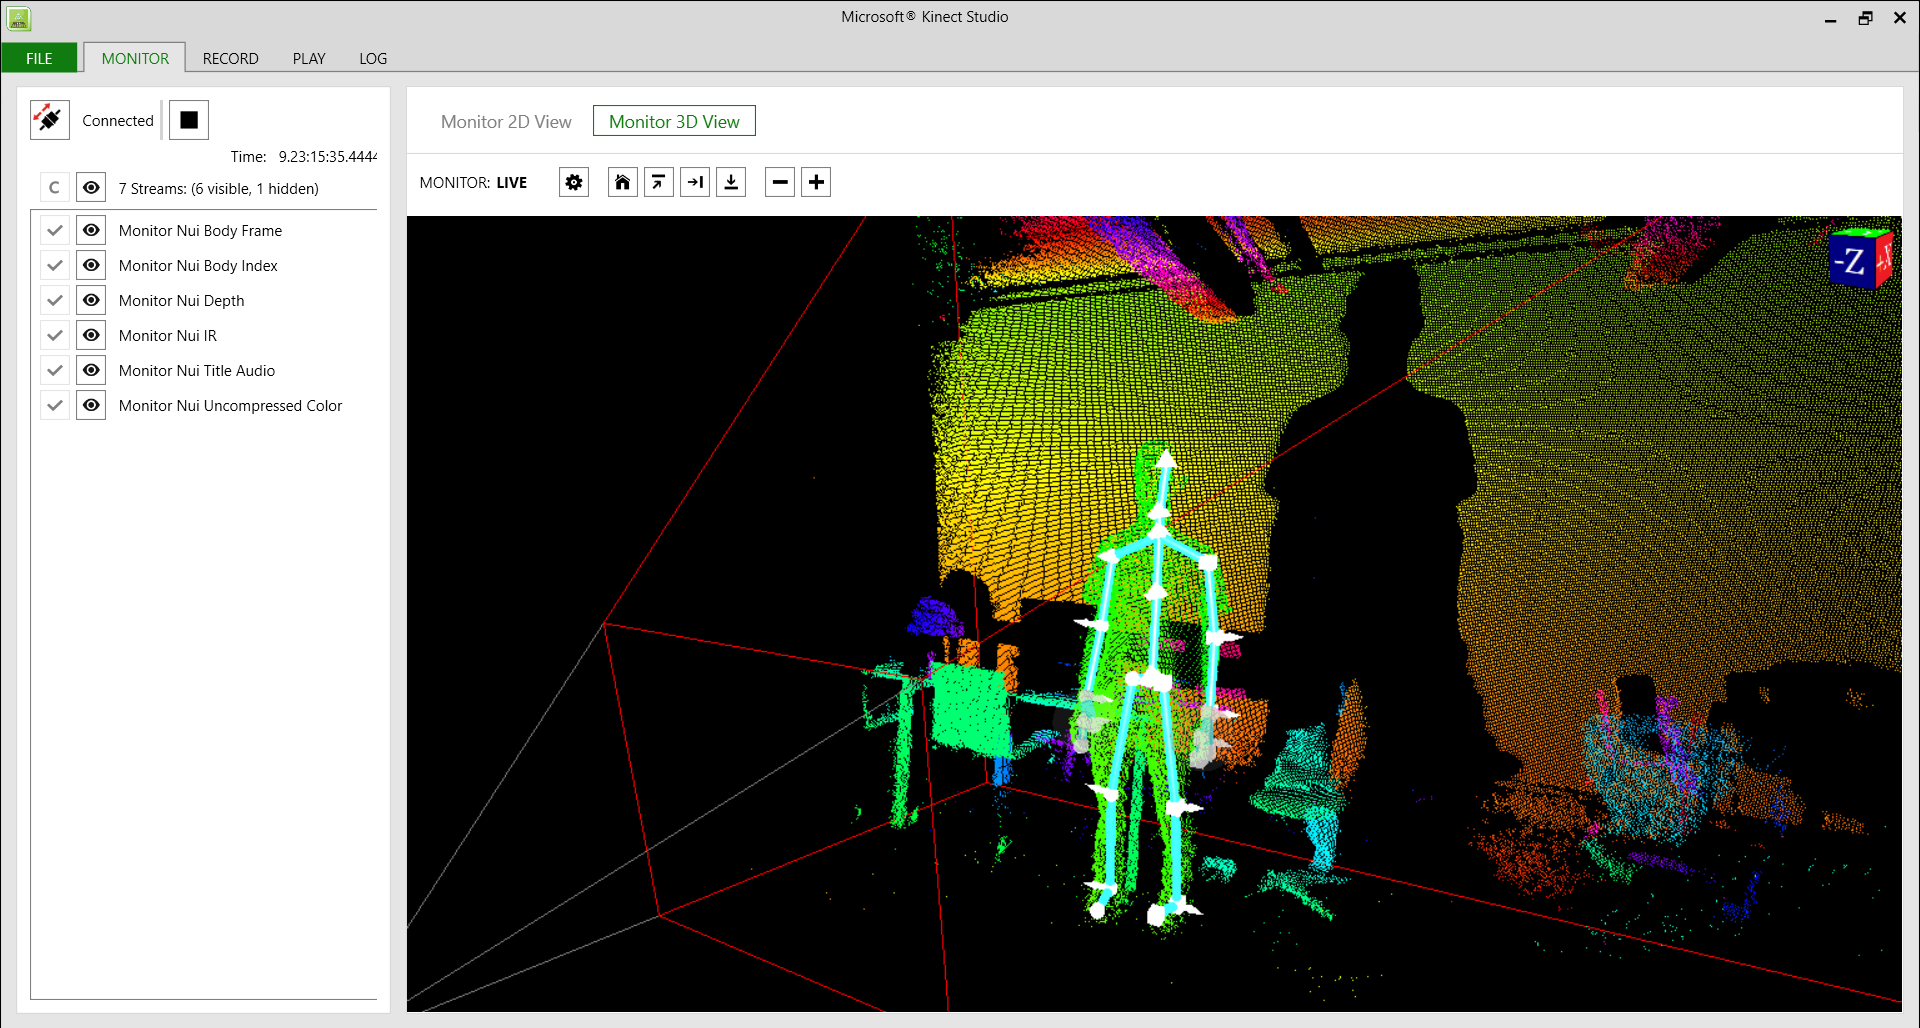
\includegraphics[width=\textwidth]{pictures/3d.png}
	\caption{Kinect-Studio mit getracktem Skelett, 3D-Ansicht.}\label{fig:studio}
	\end{figure}
	Mit dem Kinect SDK wird eine Softwarelösung namens \emph{Kinect Studio} ausgeliefert, die sich bei der Kinect-Programmierung zum visuellen Debugging eignet (siehe Abbildung \ref{fig:studio}). Im Kinect Studio können die verschiedenen Sensoraufnahmen der Kinect nebst der interpretierten Skelette und Hand-States sowie der festgestellten Tiefensituation betrachtet werden. Diese Features können getoggelt oder umgeschaltet werden. Die Tiefenkarte wird per Falschfarbendarstellung und, sofern erwünscht, sogar dreidimensional präsentiert. Ebenso kann hier die Infrarot- und Farbkameraaufnahme betrachtet werden. Das Kinect Studio erweist sich als sehr hilfreich, um die Güte der Kinect-Daten zu überprüfen und zu erkennen, ob die Kinect einen Teil des Aufnahmebereiches fehlinterpretiert. Dies ist zum Teil notwendig, um bei der Programmierung schnell und einfach zwischen Fehlern des Programmes und fehlerhaften Kinect-Daten unterscheiden zu können.
	\par
	\begin{figure}[H]
	\centering
	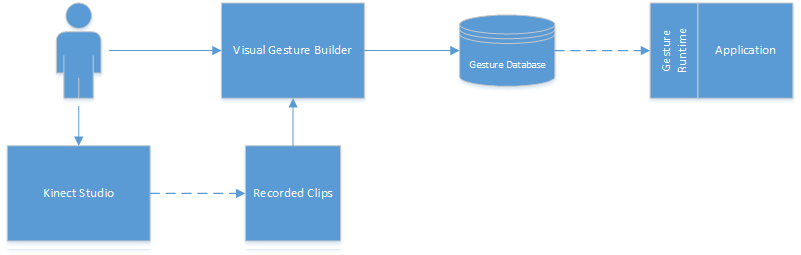
\includegraphics[width=\textwidth]{pictures/vgb.png}
	\caption{Schemadarstellung der Verwendung des \emph{Visual Gesture Builders} im Kontext eines Kinect-Programmes. Quelle: \cite{vgb}}\label{fig:vgb}
	\end{figure}
	Ebenfalls zum Kinect-SDK gehörig ist der sogenannte \emph{Visual Gesture Builder}, mit dem Gesten(folgen) aufgenommen und in Programme eingespeist werden können (siehe Abbildung \ref{fig:vgb}).
	Da die Entscheidung letztlich (siehe Abschnitt \ref{sec:gesten}) auf einen anderen Weg der Gestenimplementierung fiel, fanden hiermit nur kleinere Tests in der Anfangsphase statt.\par 
	Die Kinect-API kann mit JavaScript, C++ oder C\# verwendet werden. Da das im Rahmen der Aufgabenstellung übermittelte Programm, für das die entstehende Gestensteuerung gedacht ist, in C++ geschrieben war, wurde aus Kompatibilitäts- und Einheitlichkeitsgründen heraus ebenfalls C++ verwendet. Die Entwicklung und das Debugging fanden mit dem \emph{Microsoft Visual Studio 2015} unter \emph{Microsoft Windows 10}.\par 
	Zur Versionsverwaltung fand zusätzlich das Kommandozeilentool git mit \href{http://github.com}{GitHub} Verwendung.\par 
